\documentclass{article} % For LaTeX2e
\usepackage{nips12submit_e,times}
\usepackage{preamble}
%\usepackage{subfig}
\newcommand{\dblspace}{\setlength{\baselineskip}{0.8cm}}
\renewcommand{\pskinny}[2]{p\big(#1|#2\big)}
\usepackage{graphicx} % For figures
\usepackage{caption}
\usepackage{subcaption} 
\usepackage{natbib}   % For citations
\usepackage{algorithm}
\usepackage{algorithmic}
\usepackage{hyperref}
\newcommand{\theHalgorithm}{\arabic{algorithm}}
\usepackage[normalem]{ulem}  % for strikethrough
\usepackage{color} % for comments to each other
\usepackage{comment}
\usepackage{pgfplots}


\title{Active Learning of Model Evidence \\Using Bayesian Quadrature }

\author{
Michael A.~Osborne \\
University of Oxford\\
\texttt{mosb@robots.ox.ac.uk} \\
\And
David Duvenaud \\
University of Cambridge \\
\texttt{dkd23@cam.ac.uk} \\
\And
Roman Garnett \\
Carnegie Mellon University\\
\texttt{rgarnett@cs.cmu.edu} \\
\AND
Carl E.~Rasmussen \\
University of Cambridge \\
\texttt{cer54@cam.ac.uk} \\
\And
Stephen J.~Roberts \\
University of Oxford \\
\texttt{mosb@robots.ox.ac.uk} \\
\And
Zoubin Ghahramani \\
University of Cambridge \\
\texttt{zoubin@eng.cam.ac.uk} \\
}

% The \author macro works with any number of authors. There are two commands
% used to separate the names and addresses of multiple authors: \And and \AND.
%
% Using \And between authors leaves it to \LaTeX{} to determine where to break
% the lines. Using \AND forces a linebreak at that point. So, if \LaTeX{}
% puts 3 of 4 authors names on the first line, and the last on the second
% line, try using \AND instead of \And before the third author name.

\newcommand{\fix}{\marginpar{FIX}}
\newcommand{\new}{\marginpar{NEW}}

\nipsfinalcopy % Uncomment for camera-ready version


\begin{document} 

\maketitle

\begin{abstract} 
Numerical integration is an key component of many problems in scientific computing, statistical modelling, and machine learning. Bayesian Quadrature is a model-based method for numerical integration which, relative to standard Monte Carlo methods, offers increased sample efficiency and a more robust estimate of the uncertainty in the estimated integral. We propose a novel Bayesian Quadrature approach for numerical integration when the integrand is non-negative, such as the case of computing the marginal likelihood, predictive distribution, or normalising constant of a probabilistic model. Our approach approximately marginalises the quadrature model's hyperparameters in closed form, and introduces an active learning scheme to optimally select function evaluations, as opposed to using Monte Carlo samples. We demonstrate our method on both a number of synthetic benchmarks and a real scientific problem from astronomy.
\end{abstract} 

\section{Introduction}

The fitting of complex models to big data often requires computationally intractable integrals to be approximated. In particular, machine learning applications often require integrals over probabilities
\begin{equation}\label{eq:ev}
Z = \inty{\lfn} = \int \lfn(\vlfv) p(\vlfv) \ud\vlfv,
\end{equation}
where $\ell(\vlfv)$ is non-negative.  Examples include computing marginal likelihoods, partition functions, predictive distributions at test points, and integrating over (latent) variables or parameters in a model. While the methods we will describe are applicable to all such problems, we will explicitly consider computing model evidences, where $\ell(\vlfv)$ is the unnormalised likelihood of some parameters $x_1, \dots, x_D$. This is a particular challenge in modelling big data, where evaluating the likelihood over the entire dataset is highly computationally demanding. 

%Training or evaluating any probabilistic model typically requires an integration over model parameters, weighted by their likelihoods.  This common problem has many names:  computing the model evidence, calculating the marginal likelihood, estimating the partition function or normalizing a distribution.  Typically, this task is performed using Markov-Chain Monte Carlo (\acro{mcmc}) methods.  These methods have many well-known problems, such as requiring extensive tuning, becoming stuck in local modes, and falsely appearing to converge \cite{NealMC}.  However, almost all standard approaches fall into the wide family of \acro{mcmc} methods.

There exist several standard randomised methods for computing model evidence, such as annealed importance sampling (\acro{ais}) \cite{neal2001annealed}, nested sampling \cite{skilling2004nested} and bridge sampling.  For a review, see \cite{chen2000monte}.   These methods estimate $Z$ given the value of the integrand on a set of sample points, whose size is limited by the expense of evaluating $\ell(\vlfv)$.  It is well known that convergence diagnostics are often unreliable for Monte Carlo estimates of partition functions  \cite{NealMC, brooks1998convergence, cowles1999possible}.  Most such algorithms also have parameters which must be set by hand, such as proposal distributions or annealing schedules.

%\section{Model-Based Integration}

An alternative, model-based, approach is Bayesian Quadrature (\acro{bq}) \cite{stanford1986bayesian, BZHermiteQuadrature, kennedy1998bayesian, BZMonteCarlo}, which specifies a distribution over likelihood functions, using observations of the likelihood to infer a distribution for $Z$ (see Figure \ref{fig:model_based}). This approach offers improved sample efficiency \cite{BZMonteCarlo}, crucial for expensive samples computed on big data. We improve upon this existing work in three ways:

\begin{figure}
\centering
\psfragfig[height=3.5cm]{figures/bmc_intro6}
\caption{Model-based integration computes a posterior for the integral $Z = \int \lfn(\vlfv) p(\vlfv) \ud\vlfv$, conditioned on sampled values of the function $\lfn(\vlfv)$. For this plot, we assume a Gaussian process model for $\lfn(\vlfv)$ and a broad Gaussian prior $p(x)$. The variously probable integrands permitted under the model will give different possible values for $Z$, with associated differing probabilities.}
\label{fig:model_based}
\end{figure}

%As discussed in \cite{MCUnsound}, traditional Monte Carlo integration techniques do not make the best possible use of this valuable information. An alternative is found in Bayesian quadrature (\acro{bq}) \cite{BZHermiteQuadrature}, a method which uses function samples within a Gaussian process model to compute a closed-formed posterior over the value of the integral.



{\bf Log-GP:} \cite{BZMonteCarlo} used a \gpb prior on the likelihood function; this is a poor model, since it is unable to express the non-negativity and high dynamic range of most likelihood functions. \cite{BQR} introduced an approximate means of exploiting a \gpb on the logarithm of a function (henceforth, a log-\gp), which better captures these properties of likelihood functions. We apply this method to estimate $Z$, and extend it to compute $Z$'s posterior variance and expected variance after adding a sample. 

{\bf Active Sampling:} Previous work on \acro{bq} has used randomised or {\it a priori} fixed sampling schedules. We use active sampling, selecting locations which minimise  the expected uncertainty in $Z$.

%Our problem is to estimate the evidence of some model $M$. This is computed as 
%\begin{equation}\label{eq:ev}
% Z = p(M) = \int l(x) p(x) dx\,,
%\end{equation}
%for the likelihood $l(x) = \p{M}{x}$. The arguments $x$ represent the appropriate parameters of the model, which must be marginalised. 
%Unfortunately, the integral is typically non-analytic for interesting likelihood functions. 

{\bf Hyperparameter Marginalisation:} Uncertainty in the hyperparameters of the model used for quadrature has previously been ignored, leading to overconfidence in the estimate of $Z$.  We introduce a tractable approximate marginalisation of input scale hyperparameters.

%\paragraph*{Convergence:} Here the issue of convergence is solved naturally: our posterior variance over $Z$ indicates the uncertainty remaining in the quantity we care about. 

From a Bayesian perspective, numerical integration is fundamentally an inference and sequential decision making problem: Given a set of function evaluations, what can we infer about the integral, and how do we decide where to next evaluate the function. Monte Carlo methods, including MCMC, provide simple but generally suboptimal and non-adaptive answers: compute a sample mean, and evaluate randomly. Our approach attempts to learn about the integrand as it evaluates the function at different points, and decide based on information gain where to evaluate next. We compare our approach against standard Monte Carlo techniques and previous Bayesian approaches on both simulated and real problems.

%\section{Estimating Model Evidence}\label{sec:ev}

%Here, we give a brief overview of the standard methods used for computing nomalisation constants.  For the remainder of the paper, we will assume that we are able to draw samples from 

%Our problem is to estimate the evidence of some model $M$. This is computed as $$Z = p(M) = \int l(x) p(x) dx\,,$$ for the likelihood $l(x) = \p{M}{x}$. The arguments $x$ represent the appropriate parameters of the model, which must be marginalised. 
%Unfortunately, the integral is typically non-analytic for interesting likelihood functions. 

%\paragraph*{Annealed Importance Sampling} \cite{neal2001annealed} is a popular thermodynamic integration method which 
%These typically involve the construction of a markov chain for generating samples, leading to them being termed \emph{Markov chain Monte Carlo} (\acro{mcmc}) methods. 

%One of the main difficulties with using \acro{mcmc} methods in practice is that most methods have at least a handful of parameters which are typically set by hand. These often include a `burn-in' parameter, specifying a certain quantity of data to exclude when constructing the final estimate. The selection of this parameter can be problematic \cite{cowles1999possible}. 

%Convergence diagnostics exist to indicate if a Markov chain is failing to `mix', or explore the entire integrand.  However, these methods are known to have failure modes in which diagnostics do not identify a lack of mixing \cite{NealMC, brooks1998convergence, cowles1999possible}. One solution to this problem is found by `exact' or `perfect' sampling via coupling from the past \cite{green1999exact}, but is impractical for realistic problems. 

%While standard errors are possible for \acro{mcmc}, typically they rely on the sampler mixing well \cite{flegal2008markov}. As such, these errors can not identify exactly the failure to mix that is of most concern. The distribution of most use for our inference is a Gaussian process, which we now briefly introduce. 

\section{Gaussian Processes}
Since our \acro{bq} approach makes extensive use of Gaussian processes (\gp) \cite{GPsBook}, in this section we provide a brief introduction to \gp s and to our notation. 


A \gpb is defined as a distribution over the functions $f: \mathcal{X} \rightarrow \mathbb{R}$ such that the distribution over the possible function values on any finite subset of $\mathcal{X}$ is multivariate Gaussian. For clarity, we henceforth assume $\mathcal{X} = \mathbb{R}$, although all results generalise to $\mathbb{R}^n$. For a function $f$, the prior distribution over its vector of values $\vf$ on $\vlfv \subset \mathcal{X}$ is
\begin{align}%\label{eq:\gpbDefn}
\textstyle
 \po{\vf}\deq \N{\vf}{\vmu}{K}
 \deq\frac{1}{\sqrt{\det({2\pi K})}}\,\exp \big(-\frac{1}{2}\,(\vf-\vmu)\tra\,K\inv\,(\vf-\vmu)\big).
\end{align}
This distribution is specified by mean and covariance functions, which give the mean vector $\vmu$ and covariance matrix $K$ respectively. 
We choose Gaussian (squared exponential) covariance functions,
\begin{align} \label{eq:Gaussian_cov_fn}
% K(\vlfv,\vlfv') & \deq \prod_{e=1}^{E} K_e\big(\phi\pha_e,\phi_e'\big)\\
\textstyle
K(\lfv_1,\lfv_2)& \deq h^2\,\N{\lfv_1}{\lfv_2}{w}.
\end{align} 
Here $h$ specifies the output scale over $f$, while $w$ defines a (squared) input scale over $\lfv$. 
% Note that if $x$ has dimension greater than one, $w$ is a covariance matrix; we'll assume $w$ is diagonal. 
Given observations $(\vlfv_s,\vf_s)$, we are interested in making predictions about  $f_\star$ at input $\lfv_\star$. We will assume that function inputs such as $\vlfv_s$ and $\lfv_\star$ are always known; they will not be explicitly represented. With this information, we have the predictive equations
\begin{equation}
 \pskinny{f\st}{\vf_s} = 
\bN{f\st}
{\meancond{f}{\vlfv_\star}{s}}
{\covcond{f}{\vlfv_\star}{s}}\,,
\end{equation}
where the mean $m$, covariance $C$, and variance $V$ are
\begin{align} 
\textstyle
\meancond{f}{\lfv_\star}{s}
& \deq \mean{f_\star}{\vf_s}
= \mu(\lfv_\star)+
K(\lfv_\star,\vlfv_s)
K(\vlfv_s,\vlfv_s)\inv
\bigl(\vf_s-{\mu}(\vlfv_s)\bigr)\label{eq:GPMean}
\\[0.2cm]
C_{f|s}(\lfv_\star, \lfv'_\star)
& \deq C(f_\star,f'_\star|\vf_s) 
=K(\lfv_\star,\lfv'_\star) - 
K(\lfv_\star,\vlfv_s)
K(\vlfv_s,\vlfv_s)\inv
K(\vlfv_s,\lfv'_\star)%\label{eq:\gpbCov}
\\[0.2cm]
\covcond{f}{\lfv_\star}{s}
&\deq {\cov{f_\star}{\vf_s}} 
= C_{f|s}(\lfv_\star, \lfv_\star).
\end{align} 
Note that the above assumes implicit conditioning on hyperparameters. Where required for disambiguation, we'll make this explicit, as per $m_{f|s,w}(x\st) \deq \mean{f\st}{\vf_s, w}$ and so forth.



\section{Bayesian Quadrature} \label{sec:bq}

% Note that maximum likelihood is also subject to issues. $\p{D}{\lfv,I}$, how come (known) $I$ is on the right and (known) $D$ is on the left? 

\emph{Bayesian quadrature} \cite{BZHermiteQuadrature,BZMonteCarlo} is a means of performing Bayesian inference about the value of a potentially nonanalytic integral, $\inty{f} \deq \int f(x) p(x) \ud x$.
%Note that we use a condensed notation; this and all integrals to follow are definite integrals over the entire domain of interest.
We assume a Gaussian density
$\po{\lfv} \deq \N{\lfv}{\nu_{\lfv}}{\lambda_{\lfv}}$,
although other convenient forms, or, if necessary, the use of an importance re-weighting trick ($q(x) = \nicefrac{q(x)}{p(x)} p(x)$ for any $q(x)$), allow any other integral to be approximated. 
% If $\lfv$ is a vector, $\nu_{\lfv}$ is a  vector of identical size, and $\lambda_{\lfv}$ an appropriate covariance matrix.

%\textcolor{red}{[I'm hoping to re-write the next two paragraphs; it's way too indirect, and I think the philosophical foundations of \acro{mcmc} are a poor avenue of attack]}
Quadrature involves evaluating $f(\lfv)$ at a vector of sample points $\vlfv_s$, giving $\vf\pha_s\deq f(\vlfv_s)$. Often this evaluation is computationally expensive; the consequent sparsity of samples introduces uncertainty about the function $f$ between them, and hence uncertainty about the integral $\inty{f}$.

%As ever in the face of uncertainty, we address the estimation of the value of our integral as a problem of Bayesian inference \cite{BZNumericalAnalysis}. 

%In considering any problem of inference, we need to be clear about both what information we have and which uncertain variables we are interested in. In our case, both the values $f(\vlfv_s)$ and their locations $\vlfv_s$ represent valuable pieces of knowledge. As discussed by \cite{MCUnsound}, traditional Monte Carlo, which approximates as
%\begin{equation} \label{eq:MC_integral_estimate}
%\inty{f} \simeq \frac{1}{\card{s}} \sum_{i=1}^{\card{s}} f(\lfv_i)\,,
%\end{equation}
%effectively ignores the information content of $\vlfv_s$, leading to unsatisfactory behaviour.
%\footnote{  For example, imagine that we had $\card{s}=3$, and $\lfv_1 = \lfv_2$. In this case, the identical value $q(\lfv_1)= q(\lfv_2)$ will receive $\nicefrac{2}{3}$ of the weight, whereas the equally useful $q(\lfv_3)$ will receive only $\nicefrac{1}{3}$. \textcolor{red}{I'm not crazy about this argument, since the weightings are also incorporating information about the prior...} }

Previous work on Bayesian quadrature chooses a \gpb prior for $f$, with mean $\mu_f$ and the Gaussian covariance \eqref{eq:Gaussian_cov_fn}. Here the scales $h$ and $w$ are hyperparameters that specify the  \gpb used for Bayesian quadrature. These scales are typically fitted using type two maximum likelihood (\acro{mlii}); we will later introduce an approximate means of marginalising them in Section \ref{sec:marginalising}.

% Many more of these will be implicitly introduced in the coming sections; we'll take this as given and incorporate them into the (hidden) context $I$. 
% Note that it will later become apparent that our inference for $\inty{f}$ is independent of the $h$ quadrature hyperparameter.

Variables possessing a multivariate Gaussian distribution are jointly Gaussian distributed with any affine transformations of those variables. Because integration is affine, we can hence use computed samples $\vf_s$ to perform analytic Gaussian process inference about the value of integrals over $f(\lfv)$, such as $\inty{f}$. The mean estimate for $\inty{f}$ given $\vf_s$ is
%
\begin{align} \label{eq:mean_inty_f}
\mean{\inty{f}}{\vf_s}
& 
=\iint \inty{f}\,\p{\inty{f}}{f}\p{f}{\vf_s} \ud \inty{f} \,\ud f                                                                                                                                                               \nonumber\\
&
 =\iint \inty{f}\,\dd{\inty{f}}{\int f(\lfv)\,\po{\lfv}\,\ud\lfv}
\N{f}{\meancondfn{f}{s}}{C_{f|s}} \ud \inty{f} \,\ud f \nonumber\\
&
 = \int \meancondfn{f}{s}(\lfv)\,\po{\lfv}\,\ud\lfv
\,,
\end{align}
which is expressible in closed-form due to standard Gaussian identities \cite{BZMonteCarlo}.
%Note that the form of our `best estimate' for $\inty{f}$, \eqref{eq:mean_inty_f}, is an affine combination of the samples $\vf_s$, just as for traditional quadrature or Monte Carlo techniques. 
% Indeed, if $\mu_f$ is taken as the mean of $\vf_s$ (as is usual for \gpb inference), the second term in \eqref{eq:mean_inty_f} can be viewed as a correction factor to the Monte Carlo estimate \eqref{eq:MC_integral_estimate}. \textcolor{red}{[Since we're using a different sampling strategy than \acro{mcmc} in this paper, I think the preceeding statement is kind of misleading / confusing...]}
% \sout{Note also that $h$ represents a simple multiplicative factor to both $\ntT{s}{f}$ and $K_{f}\bigl(\vlfv_s,\vlfv_s\bigr)$, and as such cancels out of \eqref{eq:mean_inty_f}.} 
%
The corresponding closed-form expression for the posterior variance of $\inty{f}$ lends itself as a natural convergence diagnostic. Similarly, we can compute the posteriors for integrals over the product of multiple, independent functions. For example, we can calculate the posterior mean 
$\mean{\inty{f g}}{\vf_s, \vect{g}_s}$ for an integral $\int f(x) g(x) p(x) \ud x$. 
 In the following three sections, we will expand upon the improvements this paper introduces in the use of Bayesian Quadrature for computing model evidences.

\section{Modelling Likelihood Functions}\label{sec:model_lik}
%
 \begin{figure}
 \centering
 \psfragfig[height=3cm, width =8cm]{figures/log_transform2}
 \caption{A \gpb fitted to a peaked log-likelihood function  is typically a better model than \gpb fit to the likelihood function (which is non-negative and has high dynamic range). The former \gpb  also usually has the longer input scale, allowing it to generalise better to distant parts of the function. }
 \label{fig:log_is_better}
 \end{figure}
%
We wish to evaluate the evidence \eqref{eq:ev}, an integral over non-negative likelihoods, $\lfn(\lfv)$. Assigning a standard \gpb prior to $\lfn(\lfv)$ ignores prior information about the range and non-negativity of $\lfn(\lfv)$, leading to pathologies such as potentially negative evidences (as observed in \cite{BZMonteCarlo}).  A much better prior would be a \gpb prior on $\log \lfn(x)$ (see Figure \ref{fig:log_is_better}). However, the resulting integral is intractable,
\begin{equation}\label{eq:minty_l}
\mean{\If}{\vll_s}
% & 
% =\iint \inty{l}\,\p{\inty{l}}{l}\p{l}{\vl_s} \ud \inty{l} \,\ud l                                                                                                                                                               \nonumber\\
% &
 =\int \Bigl( \int \exp\bigl(\ll(\lfv)\bigr)\po{\lfv}\,\ud\lfv\Bigr)
\N{\ll}{\meancondfn{\ll}{s}}{C_{\ll|s}} \ud \ll\,,
\end{equation}
as \eqref{eq:minty_l} does not possess the affine property exploited in \eqref{eq:mean_inty_f}. To progress, we adopt an approximate inference method inspired by \cite{BQR} to tractably integrate under a log-\gpb prior.\footnote{In practice, we use the transform 
$\log\left(\lfn(\lfv) + 1\right)$, allowing us to assume the transformed quantity has zero mean. For the sake of simplicity, we omit this detail in the following derivations.} 
Specifically, we linearise the problematic exponential term around some point $\ll_0(x)$, as
\begin{equation}
 \exp\bigl(\ll(\lfv)\bigr) \simeq \exp\bigl(\ll_0(\lfv)\bigr) + \exp\bigl(\ll_0(\lfv)\bigr) \Delta(x)\label{eq:linearisation}\,
\end{equation}
where 
$
\Delta \deq \ll  - \ll_0 \,.
$
The integral \eqref{eq:minty_l} consists of the product of $Z$ and a \gpb for $\ll$; the latter, due to the light tails of the Gaussian, effectively permits only a small range of $\ll$ functions. Over this narrow region, it is reasonable to assume that $Z$ does not vary too dramatically, and can be approximated as linear in $\ll$, as is assumed by \eqref{eq:linearisation}. Using this approximation gives us
\begin{equation}\label{eq:minty_l2}
\mean{\If}{\vll_s}
 \simeq 
\mean{\If}{\ll_0, \vll_s}
\deq
\int \lfn_0(\lfv)\po{\lfv}\ud\lfv
+\int \lfn_0(\lfv)\Delta(x)\po{\lfv}\ud\lfv
\,.
\end{equation}

We now introduce a secondary \gpb model for $\lfn$, the non-log space, to assist in the linearisation of the first non-analytic integral in \eqref{eq:minty_l2}.\footnote{Although separately modelling $\lfn$ and $\log \lfn$ may seem excessive and redundant, it provides significant advantages in the  computational efficiency of the overall algorithm.} That is, we choose $\lfn_0 \deq  m_{\lfn|s}$, where $m_{\lfn|s}$ is the \gpb conditional mean (as per \eqref{eq:GPMean}) for $\lfn$ given observations $\lfn(\vlfv_s)$. For this \gpb (over the non-log space), we take zero prior means and Gaussian
covariances of the form \eqref{eq:Gaussian_cov_fn}. If a probability is dependent upon this \gpb prior, it will be represented as conditional on $\vl_s$; if dependent upon the former \gpb prior over $\ll$, it will be conditional upon $\vll_s$.
% Our linearisation corresponds to giving our \gpb over $Z$ observations
% at $\ll_0= \log (m_{r|s})$ of both the functional itself,
We expect $\Delta(\lfv)$ to be small everywhere relative to the magnitude of $\ll(x)$ (see Figure \ref{fig:delta}). Hence
 $\ll_0$ is close to the peaks of the Gaussian over $\ll$, rendering our linearisation appropriate. For $\lfn_0$, the first integral in \eqref{eq:minty_l2} becomes tractable.
\begin{figure}
\centering
\psfragfig{figures/deltav2}
\caption{Our approximate use of a \gpb for $\log \ell (x)$ improves upon the use of a \gpb for $\ell(x)$ alone.}
\label{fig:delta}
\end{figure}

Unfortunately, the second integral in \eqref{eq:minty_l2} is non-analytic due to the $\ll_0$ term within $\Delta$. As such, we perform another stage of Bayesian quadrature by treating $\Delta$ as an unknown function of $\lfv$. We use another \gpb for $\Delta$, with zero prior mean and Gaussian covariance \eqref{eq:Gaussian_cov_fn}. We must now choose \emph{candidate points} $\vlfv_c$ at which to evaluate the $\Delta$ function (note we do not need to evaluate $\lfn(\lfv_c)$ in order to compute $\Delta(\lfv_c)$).
% Unfortunately, it is impractical to resolve this decision problem in the same manner as the selection of $\vlfvS$, our ultimate goal (a topic that receives our full attention in Section \ref{sec:S\acro{bq}})).
$\vlfv_c$ should firstly include $\vlfv_s$, where we know that $\Delta$ is equal to zero. We select the remainder of $\vlfv_c$ at random on the hyper-ellipses (whose axes are defined by the input scales for $\ell$) surrounding existing observations; we expect $\delta$ to be extremised at such $\vlfv_c$. 

Given these candidates, we can now marginalise \eqref{eq:minty_l2} over $\Delta$ to give
\begin{equation} \label{eq:post_mean}
\mean{\If}{\vll_s} \simeq \mean{\If}{\ll_0,\tvr_s,\Delta_c} =
\mean{\If}{\vr_s} + \mean{\inty{\lfn \Delta}}{\vr_s, \Delta_c},
\end{equation}
where both terms are analytic as per Section \ref{sec:bq}; $\mean{\If}{\vr_s}$ is of the form \eqref{eq:mean_inty_f}. The correction factor, the second term in \eqref{eq:post_mean}, is expected to be small, since $\Delta$ is small. We extend the work of \cite{BQR} to additionally calculate the variance in the evidence,
\begin{align} 
\cov{\If}{\ll_0,\tvr_s,\Delta_c} = \secm{\If}{\ll_0,\tvr_s} - \mean{\If}{\ll_0,\tvr_s,\Delta_c}^2\,,
\end{align}
where the second moment is 
\begin{align}
\secm{\If}{\ll_0,\tvr_s} \deq  \mean{\inty{\lfn\,C_{\ll|s}\,\lfn}}{\tvr_s}+
\mean{\If}{\ll_0,\tvr_s,\Delta_c}^2,
\end{align}
and hence 
\begin{align} \label{eq:post_var}
\cov{\If}{\ll_0,\tvr_s,\Delta_c}  & = \mean{\inty{\lfn\,C_{\ll|s}\,\lfn}}{\tvr_s} \nonumber\\
& \deq
 \iint m_{\lfn|s}(\lfv) m_{\lfn|s}(\lfv') C_{\ll|s}(\lfv,\lfv')  p(x) p(x') \ud \lfv \ud\lfv',
\end{align}
which is expressible in closed form, although space precludes us from doing so. This variance can be employed as a convergence diagnostic; it describes our uncertainty in the model evidence $Z$.

In summary, we have described a linearisation approach to exploiting a \acro{gp} prior over log-likelihoods; this permitted the calculation of the analytic posterior mean \eqref{eq:post_mean} and variance \eqref{eq:post_var} of $Z$. Note that our approximation will improve with increasing numbers of samples: $\Delta$ will
eventually be small everywhere, since it is clamped to zero at each observation. 
The quality of the linearisation can also be improved by increasing the number of candidate locations, at the cost of slower computation.

\section{Marginalising hyperparameters}
\label{sec:marginalising}

We now present a novel means of approximately marginalising the hyperparameters of the \gpb used to model the log-integrand, $\ll$. In previous approaches to Bayesian Quadrature, hyperparameters were estimated using
 \acro{mlii}. However, ignoring the uncertainty in the hyperparameters can lead to pathologies. In particular, the reliability of the variance for $Z$ depends crucially upon marginalising over all unknown quantities. 

The hyperparameters of most interest are the input scales $w$ for the \gpb over the log-likelihood; these hyperparameters can have a powerful influence on the fit to a function. We use \acro{mlii} to fit all hyperparameters other than $w$. Marginalisation of $w$ is confounded by the complex dependence of our predictions upon these input scales. 
% However, any approximation we make is likely to improve upon the assumption made by \acro{mlii}: that the posterior for all hyperparameters is a delta function. 
We make the following essential assumptions:

{\bf Flat prior:} We assume that the prior for $w$ is broad, so that our posterior is the normalised likelihood.

{\bf Laplace approximation:} The likelihood of $w$ is taken as Gaussian with mean equal to the \acro{mlii} value $\hat{w}$ and with diagonal covariance $C_w$, diagonal elements fitted using the second derivatives of the likelihood. We represent the posterior mean for $\ll$ conditioned on $\hat{w}$ as $\hat{m} \deq m_{\ll|s,\hat{w}}$.

{\bf GP mean affine in $w$:} Given the narrow width of the likelihood for $w$, our predictions for $\ll$ are assumed to have a \gpb mean which is affine in $w$ around the \acro{mlii} values, and a constant covariance;
$m_{\ll|s,w} \simeq \hat{m}
 + \pderiv{\hat{m} }{w} (w- \hat{w})$
and
$
C_{\ll|s, w} \simeq C_{\ll|s, \hat{w}}.
$
 
The implication of these assumptions is that the marginal posterior mean over $\ll$ is simply
$
\tilde{m}_{\ll|s} \deq m_{\ll|s,\hat{w}}
$.   
The marginal posterior variance is 
$
\tilde{C}_{\ll|s} 
\deq C_{\ll|s,\hat{w}}
+ 
\pderiv{\hat{m}}{w}
\,C_w\,
\pderiv{\hat{m}}{w}\,.
$
%which is identical to \eqref{eq:mean_ev} (note that we had previously just implicitly assumed that $\theta=\hat{w}$). 
%
\begin{figure}
	\begin{subfigure}[b]{6cm}
		\psfragfig[height = 4cm, width = 6cm]{figures/int_hypers2}
		\caption{}
		\label{fig:integrate_hypers}
	\end{subfigure}
\hspace{-1cm}
	\begin{subfigure}[b]{8cm}
		\psfragfig[height = 4cm, width = 8cm]{figures/eue_progression2}
		\caption{}
		 \label{fig:eue}
	\end{subfigure}
\caption{\subref{fig:integrate_hypers}) Integrating hyperparameters increases the marginal posterior variance (in regions whose mean varies as the input scales change) to more closely match the true posterior marginal variance. \subref{fig:eue}) An example showing the expected uncertainty in the evidence after observing the likelihood function at that location. $p(x)$ and $l(x)$ are plotted at the top in green and black respectively, the next sample location in red.  Note the model discovering a new mode on the right hand side, sampling around it, then moving on to other regions of high uncertainty on the left hand side. }
\end{figure}
%
%
An example of our approximate posterior is depicted in Figure  \ref{fig:integrate_hypers}.
Our approximations give the marginal posterior mean for $Z$:
\begin{equation}
\tilde{m}(\If|\ll_0,\tvr_s,\Delta_c) \deq \mean{\If}{\ll_0,\tvr_s,\Delta_c, \hat{w}}\,,
\end{equation}
of the form \eqref{eq:post_mean}. The marginal posterior variance
\begin{align}
\tilde{V}(\If|\ll_0,\tvr_s,\Delta_c)=
\iint\ud \lfv\, \ud\lfv' m_{\lfn|s}(\lfv)\, m_{\lfn|s}(\lfv') 
\biggl(C_{\ll|s}(\lfv,\lfv') + 
\pderiv{\hat{m}(x)}{w}
\,C_w\,
\pderiv{\hat{m}(x')}{w}
\biggr)
\end{align}
is possible, although laborious, to express analytically, as with \eqref{eq:post_var}. 

%Figure \ref{fig:integrate_hypers} demonstrates our approximate marginalisation on a simple example.

\section{Active Sampling}\label{sec:BBQ}

One major benefit of model-based integration is that samples can be chosen by any method, in contrast to Monte Carlo methods, which typically must sample from a specific distribution.  In this section, we describe a scheme to select samples $\lfv_s$ sequentially, by minimising the \textit{expected} uncertainty in the evidence that remains after taking each additional sample.\footnote{We also expect such samples to be useful not just for estimating the evidence, but also for any other related expectations, such as would be required to perform prediction using the model.} We take the variance in the evidence as our loss function, and proceed according to Bayesian decision theory.

Surprisingly, the posterior variance of a \gpb model with fixed hyperparameters does not depend on the function values at sampled locations at all; only the location of those samples matters. In traditional Bayesian quadrature, the evidence is an affine transformation of the sampled likelihood values, hence its estimate for the variance in the evidence is also independent of likelihood values. As such, active learning with fixed hyperparameters is pointless, and the optimal sampling design can be found in advance \cite{minka2000dqr}.

In Section \ref{sec:model_lik}, we took $Z$ as an affine transform of the log-likelihood, which we model with a \gp. As the affine transformation \eqref{eq:linearisation} itself depends on the function values, active learning is  desirable. The uncertainty over the hyperparameters of the \gpb further motivates active learning: without assuming \textit{a priori} knowledge of the hyperparameters, we can't evaluate the \gpb to precompute a sampling schedule. The approximate marginalisation of hyperparameters permits an approach to active sampling that acknowledges the influence new samples may have on the posterior over hyperparameters. 
 
%\begin{figure}
%\centering
%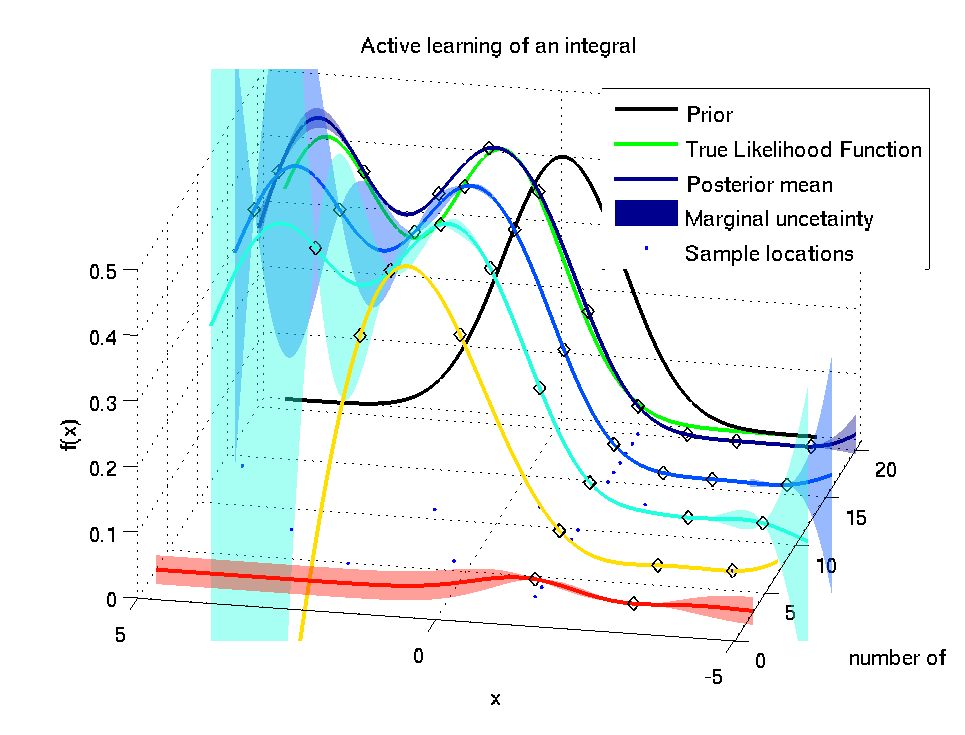
\includegraphics[width=0.48\textwidth]{figures/active_learning.eps}
%\caption{An example of the posterior over likelihood functions converging as new samples are selected.}
%\label{fig:active_learning}
%\end{figure}
% 
% \begin{figure}
% \centering
% \psfragfig{figures/plots/sampleplot_two_spikes_1d}
% \caption{The location of samples chosen by different methods.}
% \label{fig:sample_paths}
% \end{figure}

Active sampling selects a new sample $\lfv_a$ so as to minimise the expected variance in the evidence after adding the sample to the model of $\ell$.  The objective is therefore to choose the $\lfv_a$ that minimises the expected loss;
$\lfv_a = \argmin_{\lfv_a} \bigl\langle \cov{\If}{\ll_0,\tvr_{s,a}}\mid \ll_0,\tvr_{s}\bigr\rangle 
$
(note $x_a$ is implicitly conditioned on, as usual for function inputs) where the expected loss is
\begin{align}
\bigl\langle \cov{\If}{\ll_0,\tvr_{s,a}}\mid \ll_0,\tvr_{s}\bigr\rangle 
% & = \secm{\inty{\lfn}}{\ll_0,\tvr_s} 
% - \int\mean{\inty{\lfn}}{\ll_0,\tvr_{a,s},\Delta_c}^2\nonumber\\
% & \hspace{3.8cm} \p{\ll_a}{\tvr_s}\ud\ll_a\,.\nonumber\\
 & = \secm{\If}{\ll_0,\tvr_s} 
 - \int\mean{\If}{\ll_0,\tvr_{a,s},\Delta_c}^2\nonumber\\
& \hspace{0.3cm}
\times\N{\ll_a}
{\hat{m}_a }
{\hat{C}_a +\pderiv{\hat{m}_a}{w}C_w\pderiv{\hat{m}\tra_a}{w}}
\ud\ll_a\,,\label{eq:exp_var}
\end{align}
and we define
$\hat{m}_a \deq \mean{\ll_a}{\tvr_s,\hat{w}}$
and
$\hat{C}_a \deq \cov{\ll_a}{\tvr_s,\hat{w}}$.
The first term in \eqref{eq:exp_var}, the second moment, is independent of the selection of $\lfv_a$ and can hence  be safely ignored for active sampling (true regardless of the model chosen for the likelihood). 
The second term, the negative expected squared mean, can be resolved analytically\footnote{Here we use the fact that $\int \exp(c\, y)\, \N{y}{m}{\sigma^2} \ud y = \exp(c\, m + \nicefrac{1}{2}\, c^2 \sigma^2)$.  We assume that $\Delta$ does not depend on $\ll_a$, only its location $x_a$: we know $\Delta(x_a) = 0$ and assume $\Delta$ elsewhere remains unchanged.}
 for any trial $\lfv_a$ (we omit the laborious details). 

Importantly, we do not have to make a linearisation approximation here. That is, the \gpb  posterior over $\ll_a$ can be fully exploited when performing active sampling.
%

In order to minimise the expected variance, the objective in \eqref{eq:exp_var} encourages the maximisation of the expected squared mean of $Z$. Due to our log-\gpb model, one means the method can use to do this is to seek points where the log-likelihood is predicted to be large: which we call \emph{exploitation}.  The objective in \eqref{eq:exp_var} naturally balances exploitation against \emph{exploration}: the choice of points where our current variance in the log-likelihood is significant (see Figure \ref{fig:eue}). Note that the variance for $\ll_a$ is increased by approximate integration over hyperparameters, encouraging exploration.

\section{Experiments}
\label{sec:experiments}



We now present empirical evaluation of our algorithm in a variety of different experiments.

\paragraph{Metrics:} We judged our methods according to three metrics, all averages over $N$ similar experiments indexed by $i$. Define $Z_i$ as the ground truth evidence for the $i$th experiment, $m(Z_i)$ as its estimated mean  and $V(Z_i)$  as its predicted variance. Firstly, we computed the average log error,
$
\acro{ale} 
\deq \frac{1}{N} \sum_{i=1}^{N} \left|{\log m(Z_i) - \log Z_i}\right|\,.
$
Next we computed the negative log-density of the truth, assuming experiments are independent,
$
-\log p(\vect{Z}) = -\sum_{i=1}^{N} \log \N{Z_i}{m(Z_i)}{V(Z_i)}
$, which quantifies the accuracy of our variance estimates. We also computed the calibration $\mathcal{C}$, defined as the fraction of experiments in which the ground truth lay within our 50\% confidence interval $\bigl(m(Z_i) - 0.6745 \surd{V(Z_i)}, m(Z_i) + 0.6745 \surd{V(Z_i)}\bigr)$. Ideally, $\mathcal{C}$ would be  50\%: any higher, and a method is under-confident, any lower and it is over-confident. 

\paragraph{Methods:} We first compared against simple Monte Carlo (\acro{smc}). \acro{smc} generates samples $x_1, \dots, x_N$ from $p(x)$, and estimates $Z$ by $\hat{Z} = \nicefrac{1}{N} \sum_{n=1}^{N} \lfn(x_n)$.  An estimate of the variance of $\hat{Z}$ is given by the standard error of $\lfn({\bf x})$. As an alternative Monte Carlo technique, we implemented Annealed Importance Sampling (\acro{ais}) using a Metropolis-Hastings sampler.  The inverse temperature schedule was linear as in \cite{BZMonteCarlo}, and the proposal width was adjusted to attain approximately a 50\% acceptance rate. Note that a single \acro{ais} chain provides no ready means of determining the posterior variance for its  estimate of $Z$.  
% An alternative sampler is Hamiltonian Monte Carlo, which uses information about the derivatives in order to speed mixing.  However, Bayesian Quadrature can also incorporate information about the derivatives of the likelihood function, and would presumably also perform better if given this information.  An exhaustive comparison of sampling methods is beyond the scope of this paper.
Our first model-based method was Bayesian Monte Carlo (\acro{bmc}) -- the algorithm used in \cite{BZMonteCarlo}. Here samples were drawn from the \acro{ais} chain above, and a \gpb was fit to the likelihood samples. For this and other methods, where not otherwise mentioned, \gpb hyperparameters were selected using \acro{mlii}. 

We then tested four novel methods. Firstly, Bayesian Quadrature (\acro{bq}), which employed the linearisation approach of Section \ref{sec:model_lik} to modeling the log-transformed likelihood values. The samples supplied to it were drawn from the same \acro{ais} chain as used above, and 400 candidate points were permitted. \acro{bq}* is the same algorithm as \acro{bq} but with hyperparameters approximately marginalised, as per Section \ref{sec:marginalising}. Note that this influences only the variance of the estimate; the means for \acro{bq} and \acro{bq*} are identical. The performance of these methods allow us to quantify to what extent our innovations improve estimation given a fixed set of samples. 

Next, we tested a novel algorithm, Doubly Bayesian Quadrature (\acro{bbq}). The method is so named for the fact that we use not only Bayesian inference (with a \gpb over the log-transformed likelihood) to compute the posterior for the evidence, but also Bayesian decision theory to select our samples actively, as described in Section \ref{sec:BBQ}. %Note that \eqref{eq:exp_var} was minimised using a multi-start local optimiser, where the starting points were chosen both near the current likelihood maximum, for exploitation, and as draws from the prior, for exploration.
\acro{bbq}* is identical, but with hyperparameters approximately marginalised. Both algorithms demonstrate the influence of active sampling on our performance. 

\paragraph{Problems:}
We used these methods to evaluate evidences given Gaussian priors and a variety of likelihood functions. As in \cite{BZMonteCarlo} and \cite{BQR}, we focus on low numbers of samples; we permitted tested methods 150 samples on synthetic integrands, and 300 when using real data. We are motivated by real-world, big-data, problems where evaluating likelihood samples is expensive, making it desirable to determine the techniques for evidence estimation that can operate best when permitted only a small number of samples. Ground truth $Z$ is available for some integrals; for the non-analytic integrals, $Z$ was estimated by a run of \acro{smc} with $10^5$ samples.

We considered seven synthetic examples. We firstly tested using single Gaussians, in one, four, ten and twenty dimensions. We also tested on mixtures of two Gaussians in one dimension (two examples, alternately widely separated and overlapping) and four dimensions (a single example). %In dimension greater than four, the great difficulty of 

We additionally tested methods on a real scientific problem: detecting a damped Lyman-$\alpha$ absorber (\textsc{dla}) between the Earth and
an observed quasar from spectrographic readings of the quasar.
\textsc{dla}s are large objects consisting primarily
of neutral hydrogen gas.  
The statistical properties of \textsc{dla}s inform us about the distribution of neutral hydrogen in the
universe, which is of fundamental cosmological importance. We model the quasar spectra using a \gp; the presence
of a \textsc{dla} is represented as an observation fault with known dynamics \citep{garnett2010sequential}. This model has five hyperparameters to be marginalised, to which we assign priors drawn from the large corpus of data obtained from the Sloan Digital Sky Survey (\acro{sdss}) \citep{sdss}. We tested over four datasets; the expense of evaluating a \gpb likelihood sample on the large datasets available from the \acro{sdss} (140TB of data have been released in total) motivates the small sample sizes considered.




\paragraph{Evaluation}

%  \begin{figure}
%  \centering
%  \begin{tabular}{ccc}
%  	\psfragfig{figures/integrands/easy_1d} &
%  	\psfragfig{figures/integrands/bumpy_1d} 
%  	\psfragfig{figures/integrands/two_spikes_1d}
%  \end{tabular}
%  \caption{The one-dimensional integrands in our test suite.  Green dashed lines are priors, blue lines are likelihoods.
%  % \textcolor{red}{mike says: maybe we should make the lines variously dashed to help with B\&W printing. Also I'm not sure we need the posterior, which could be removed to de-clutter.}
%  }
%  \label{fig:1d_problems}
%  \end{figure}
% 
% %\begin{figure}
% %\centering
% %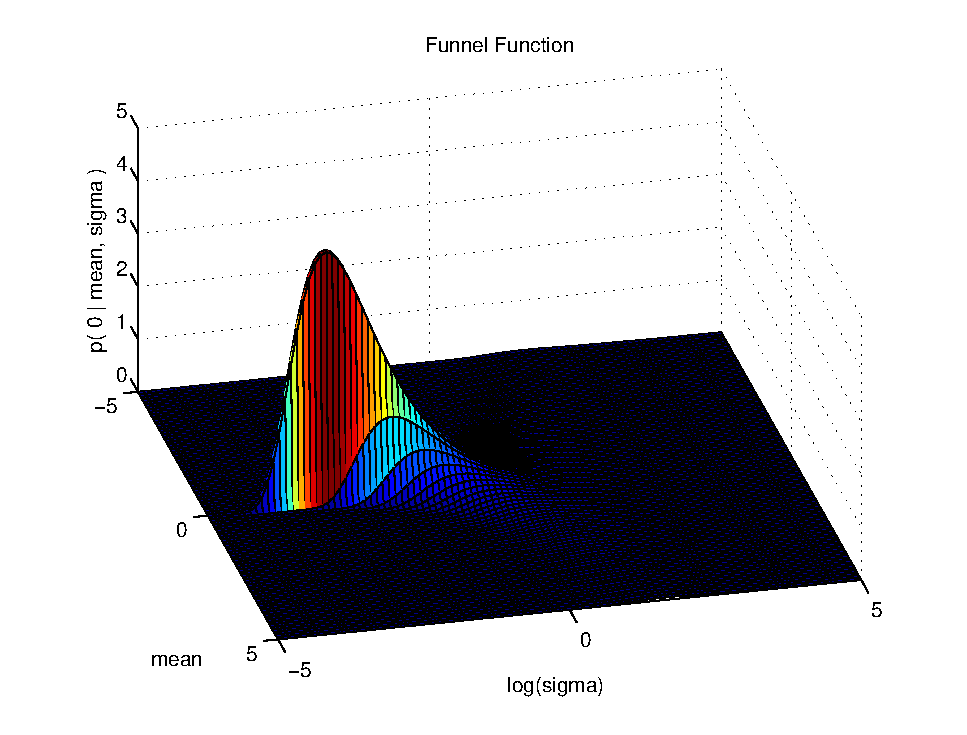
\includegraphics[width=0.45\textwidth]{figures/integrands/funnel.eps}
% %\caption{Radford Neal's funnel problem in 2 dimensions.}
% %\label{fig:funnel}
% %\end{figure}
% 
% %\begin{minipage}[t][0.45\paperheight][t]{0.45\paperwidth}
% %    % --- Automatically generated by latex_table.m ---
% Exported at 16-Feb-2012 13:24:18
\begin{table}[h!]
\caption{{\small
time taken (s)
}}
\label{tbl:time taken (s)}
\begin{center}
\begin{tabular}{l  r r r r r r r}
Integrand & \rotatebox{0}{ SMC }  & \rotatebox{0}{ AIS }  & \rotatebox{0}{ BMC AIS }  & \rotatebox{0}{ LBMC }  & \rotatebox{0}{ SBQ }  & \rotatebox{0}{ SBQ GPML }  & \rotatebox{0}{ BQ AIS }  \\ \midrule
simple & $\mathbf{0.023}$ & $1.306$ & $2.026$ & $1.251$ & $36.344$ & $12.158$ & $22.325$ \\
simple translated & $\mathbf{0.009}$ & $1.295$ & $1.948$ & $1.384$ & $ NaN$ & $ NaN$ & $23.192$ \\
simple scaled & $\mathbf{0.012}$ & $1.288$ & $1.897$ & $1.116$ & $37.762$ & $11.947$ & $21.611$ \\
easy 1d & $\mathbf{0.009}$ & $1.766$ & $2.064$ & $1.079$ & $45.821$ & $12.779$ & $ NaN$ \\
bumpy 1d & $\mathbf{0.007}$ & $1.126$ & $2.119$ & $1.144$ & $16.984$ & $26.335$ & $35.352$ \\
two spikes 1d & $\mathbf{0.016}$ & $2.781$ & $2.342$ & $1.888$ & $45.635$ & $ NaN$ & $45.693$ \\
two hills 1d & $\mathbf{0.020}$ & $2.781$ & $2.151$ & $1.091$ & $38.483$ & $11.402$ & $30.592$ \\
funnel 2d & $\mathbf{0.033}$ & $2.566$ & $2.241$ & $0.618$ & $67.442$ & $6.688$ & $9.770$ \\
friedman 3d & $\mathbf{0.371}$ & $12.441$ & $3.578$ & $0.447$ & $171.890$ & $7.807$ & $11.814$ \\
easy 4d & $\mathbf{0.010}$ & $1.924$ & $2.518$ & $0.666$ & $147.084$ & $10.071$ & $11.208$ \\
two spikes 4d & $\mathbf{0.012}$ & $2.997$ & $2.829$ & $ NaN$ & $ NaN$ & $ NaN$ & $ NaN$ \\
two hills 4d & $\mathbf{0.012}$ & $2.984$ & $2.321$ & $0.637$ & $219.580$ & $16.164$ & $11.057$ \\
friedman 7d & $\mathbf{0.356}$ & $11.618$ & $3.990$ & $4.756$ & $443.423$ & $57.409$ & $ NaN$ \\
\end{tabular}
\end{center}
\end{table}
% End automatically generated LaTeX

% %\end{minipage}
% 
% 
%\begin{figure}
%	\centering
%\end{figure}

\begin{figure}
%	\centering
	\begin{subfigure}[b]{7.5cm}
		\psfragfig[width=5cm,height=2.5cm]{figures/plots/varplot_two_spikes_1d_nice1} 	
		\psfragfig[width=3cm, height=3cm]{figures/plots/legend}
		\caption{}
		\label{fig:se}
	\end{subfigure}
	\begin{subfigure}[b]{6cm}
		\psfragfig[width=6cm,height=2.5cm]{figures/plots/log_of_truth_plot_two_hills_1d_nice1}
		\caption{}
		\label{fig:nll}
	\end{subfigure}
	\caption{\subref{fig:se}) The posterior distribution over $Z$ for several methods on a one-dimensional example as the number of samples increases.  Shaded regions denote $\pm2$ \acro{sd}'s from the mean.  The shaded regions for \acro{smc} and \acro{bmc} are off the vertical scale of this figure. \subref{fig:nll}) The log density of the true evidence for different methods (colours identical to those in \subref{fig:se}), compared to the true $Z$ (in black).  The integrand is the same as that in Figure \ref{fig:eue}.}
\end{figure}

\begin{table}[h!]
\begin{minipage}[b]{0.5\linewidth}\centering
% --- Automatically generated by latex_table.m ---
% Exported at 24-Feb-2012 23:39:08
\begin{table}[h!]
\caption{{\small
Combined Synthetic Results
}}
\label{tbl:Combined Synthetic Results}
\begin{center}
\begin{tabular}{l  r r r}
Method & \rotatebox{0}{ $-\log p(\mathbf{Z})$ }  & \rotatebox{0}{ \acro{RMNSE} }  & \rotatebox{0}{ $\mathcal{C}$ }  \\ \midrule
\acro{\lowercase{SMC}} & $-1.201$ & $0.262$ & $0.500$ \\
\acro{\lowercase{AIS}} & N/A & $0.585$ & N/A \\
\acro{\lowercase{BMC}} & $2.410$ & $0.265$ & $0.625$ \\
\acro{\lowercase{BQ}} & $3.081$ & $0.296$ & $0.625$ \\
\acro{\lowercase{BQ*}} & $3.067$ & $0.296$ & $0.625$ \\
\acro{\lowercase{BBQ*}} & $>$ 1000 & $0.554$ & $0.375$ \\
\acro{\lowercase{BQ}} & $3.067$ & $0.296$ & $0.625$ \\
\acro{\lowercase{BBQ}} & $25.383$ & $0.298$ & $0.375$ \\
\acro{\lowercase{BBQ*}} & $\mathbf{-13.747}$ & $\mathbf{0.102}$ & $0.625$ \\
\end{tabular}
\end{center}
\end{table}
% End automatically generated LaTeX

\end{minipage}
%\hspace{0.5cm}
\begin{minipage}[b]{0.5\linewidth}\centering
\input{tables/combined_dla.tex}
\end{minipage}
%% --- Automatically generated by latex_table.m ---
% Exported at 24-Feb-2012 14:59:39
\begin{table}[h!]
\caption{{\small
Combined Prawn Results
}}
\label{tbl:Combined Prawn Results}
\begin{center}
\begin{tabular}{l  r r r}
Method & \rotatebox{0}{ $-\log p(\mathbf{Z})$ }  & \rotatebox{0}{ \acro{rmnse} }  & \rotatebox{0}{ $\mathcal{C}$ }  \\ \midrule
\acro{smc} & $>$ 1000 & $1.067$ & $0.333$ \\
\acro{ais} & N/A & $0.909$ & N/A \\
\acro{bmc} & $7.300$ & $1.107$ & $0.667$ \\
\acro{bq} & $6.996$ & $1.040$ & $0.333$ \\
\acro{bq*} & $\mathbf{6.918}$ & $1.040$ & $0.333$ \\
\acro{bbq} & $>$ 1000 & $0.933$ & $0.000$ \\
\acro{bbq*} & $>$ 1000 & $\mathbf{0.861}$ & $0.000$ \\
\end{tabular}
\end{center}
\end{table}
% End automatically generated LaTeX

\end{table}

Table \ref{tbl:Combined Synthetic Results} shows combined performance on the synthetic integrands listed above. The calibration scores $\mathcal{C}$ show that all methods\footnote{Because a single \acro{ais} chain gives no estimate of uncertainty, it has no likelihood or calibration scores.} are systematically overconfident, although our approaches are at least as well calibrated as alternatives. On average, \acro{bbq*} provides an estimate of $Z$ which is closer to the truth than the other methods given the same number of samples, and assigns much higher likelihood to the true value of $Z$. \acro{bbq*} also achieved the lowest error on five, and best likelihood on six, of the seven problems, including the twenty dimensional problem for both metrics.  Figure \ref{fig:se} shows a case where both
 \acro{smc} and \acro{bbq*} are relatively close to the true value, however \acro{bbq*}'s posterior variance is much smaller.  Figure \ref{fig:nll} demonstrates the typical behavior of the active sampling of \acro{bbq*}, which quickly concentrates the posterior distribution at the true $Z$. The negative likelihoods of \acro{bq*} are for every problem slightly lower than for \acro{bq} ($-\log p(\mathbf{Z})$ is on average $0.2$ lower), indicating that the approximate marginalisation of hyperparameters grants a small improvement in variance estimate. 

Table \ref{tbl:Combined Real Results} shows results for the various methods on the real integration problems. Here \acro{bbq} is clearly the best performer; the additional exploration induced by the hyperparameter marginalisation of \acro{bbq*} may have led to local peaks being incompletely exploited. Exploration in a relatively high dimensional, multi-modal space is inherently risky; nonetheless, \acro{bbq*} achieved lower error than \acro{bbq} on two of the problems.
%Here, we see that although \acro{bbq*} was again closest on average to the truth, it was overconfident.  The method that gave the highest likelihood to the true $Z$ was one which did not perform active sampling, but obtained samples through an \acro{ais} chain.  This is likely due to the stationarity assumption made by our \gpb model, which sometimes leads to overconfident extrapolation.

%The relative performances of \acro{bbq} and \acro{bbq*} reveal that this marginalisation forms a significant contribution to the effective selection of samples. 

\section{Conclusions}

 In this paper, we have made several advances to the \acro{bq} method for evidence estimation.  These are: approximately imposing a positivity constraint, approximately marginalising hyperparameters, and using active sampling to select the location of function evaluations. Of these contributions, the active learning approach yielded the most significant gains for integral estimation.
 
 
%   We  have demonstrated the superior sample efficiency of an active learning approach to integral estimation.
% \acro{mc} is an extremely widely used method, and advances in  allow modelers to use richer model classes and to be more confident in their model evaluations.  
%We hope that thse contributions expect that the class of model-based quadrature approaches will come to be seen as a viable alternative to \acro{mc} for some problem classes.

% Adjusting the number of candidate points allows one to trade off between computational speed and number of samples required.

% While we used an active learning scheme in this paper, Bayesian Quadrature can be used on samples generated by any method.

%There are many ways to improve the \gpb model used to model likelihood functions.  Notably, the Gaussian kernel used in this paper has very weak generalization abilities;  allowing a richer class of kernels might permit the \gpb model to shrink its posterior more quickly. With other covarances, the methods developed here can also be readily applied to discrete domains.
% For example, log-likelihood functions typically take the form of a sum of many terms, each depending only on a small number of variables.  This prior information could easily be incorporated into the \gp, presumably allowing the \acro{bbq} algorithm to form concentrated posterior distributions over high-dimensional likelihoods.


\subsubsection*{Acknowledgements}
\small
\acro{m.a.o.} was funded by the \acro{orchid} project (\url{http://www.orchid.ac.uk/}).

\pagebreak
\bibliography{bub}
\bibliographystyle{unsrt}
%\pagebreak
%% --- Automatically generated by latex_table.m ---
% Exported at 11-Feb-2012 20:59:11
\begin{table}[h!]
\caption{{\small
neg log density of truth at 100 samples
}}
\label{tbl:neg log density of truth at 100 samples}
\begin{center}
\begin{tabular}{l  r r r r r r}
Integrand & \rotatebox{0}{ SMC }  & \rotatebox{0}{ AIS }  & \rotatebox{0}{ BMC }  & \rotatebox{0}{ SBQ }  & \rotatebox{0}{ SBQ GPML }  & \rotatebox{0}{ BQ GPML AIS }  \\ \midrule
simple test & $-1.186$ & $233.335$ & $\mathbf{-2.942}$ & $-2.237$ & $-0.999$ & $-1.915$ \\
simple test transformed & $-1.186$ & $233.335$ & $\mathbf{-2.942}$ & $ NaN$ & $-1.104$ & $-1.915$ \\
easy 1d & $0.627$ & $\mathbf{-2.198}$ & $-1.189$ & $-0.453$ & $-1.145$ & $-1.353$ \\
bumpy 1d & $\mathbf{-3.050}$ & $>$ 1000 & $3.163$ & $-2.043$ & $ NaN$ & $0.867$ \\
bumpy 1d exp & $\mathbf{-3.518}$ & $>$ 1000 & $0.731$ & $-2.424$ & $ NaN$ & $0.015$ \\
two spikes 1d & $2.970$ & $24.156$ & $1.386$ & $ NaN$ & $\mathbf{0.120}$ & $1.220$ \\
two hills 1d & $2.970$ & $24.156$ & $1.386$ & $ NaN$ & $\mathbf{0.120}$ & $1.220$ \\
funnel 2d & $12.439$ & $52.654$ & $\mathbf{0.493}$ & $ NaN$ & $ NaN$ & $0.782$ \\
friedman 3d & $\mathbf{ NaN}$ & $ NaN$ & $ NaN$ & $ NaN$ & $ NaN$ & $ NaN$ \\
easy 4d & $0.601$ & $44.220$ & $0.410$ & $ NaN$ & $ NaN$ & $\mathbf{0.328}$ \\
two spikes 4d & $\mathbf{5.977}$ & $153.904$ & $23.489$ & $ NaN$ & $ NaN$ & $13.897$ \\
two hills 4d & $2.741$ & $687.308$ & $21.552$ & $ NaN$ & $ NaN$ & $\mathbf{0.356}$ \\
friedman 7d & $\mathbf{ NaN}$ & $ NaN$ & $ NaN$ & $ NaN$ & $ NaN$ & $ NaN$ \\
\end{tabular}
\end{center}
\end{table}
% End automatically generated LaTeX

%% --- Automatically generated by latex_table.m ---
% Exported at 24-Feb-2012 15:01:01
\begin{table}[h!]
\caption{{\small
log squared error at 150 samples
}}
\label{tbl:log squared error at 150 samples}
\begin{center}
\begin{tabular}{l  r r r r r r r}
Integrand & \rotatebox{0}{ SMC }  & \rotatebox{0}{ AIS }  & \rotatebox{0}{ BMC }  & \rotatebox{0}{ BQ }  & \rotatebox{0}{ BQ* }  & \rotatebox{0}{ BBQ }  & \rotatebox{0}{ BBQ* }  \\ \midrule
simple & $-5.713$ & $-0.758$ & $-10.933$ & $-10.336$ & $-10.336$ & $-13.335$ & $\mathbf{-14.468}$ \\
bumpy 1d & $-4.859$ & $-6.866$ & $-3.286$ & $-3.466$ & $-3.466$ & $-2.594$ & $\mathbf{-10.106}$ \\
two spikes 1d & $-1.294$ & $\mathbf{-5.449}$ & $-0.821$ & $-0.574$ & $-0.574$ & $-1.724$ & $-3.628$ \\
two hills 1d & $-9.423$ & $-2.346$ & $-5.229$ & $-14.669$ & $-14.669$ & $\mathbf{-18.318}$ & $-18.317$ \\
funnel 2d & $-3.921$ & $-0.070$ & $-1.467$ & $-1.437$ & $-1.437$ & $-2.206$ & $\mathbf{-4.454}$ \\
easy 4d & $-6.665$ & $-4.655$ & $-4.073$ & $\mathbf{-6.785}$ & $-6.785$ & $-1.909$ & $-5.237$ \\
two spikes 4d & $-2.030$ & $3.664$ & $-3.540$ & $-2.275$ & $-2.275$ & $-2.322$ & $\mathbf{-4.772}$ \\
two hills 4d & $-0.707$ & $2.858$ & $-1.909$ & $-1.265$ & $-1.265$ & $-2.725$ & $\mathbf{-3.543}$ \\
real prawn 6d mean field & $\mathbf{-7.259}$ & $2.173$ & $-1.416$ & $-1.187$ & $-1.187$ & $2.084$ & $2.083$ \\
real prawn 6d markov & $\mathbf{-5.056}$ & $3.795$ & $3.000$ & $3.028$ & $3.028$ & $3.408$ & $3.412$ \\
real prawn 6d non-markov & $\mathbf{3.621}$ & $4.499$ & $3.710$ & $3.642$ & $3.642$ & $4.343$ & $4.346$ \\
\end{tabular}
\end{center}
\end{table}
% End automatically generated LaTeX


\end{document} 



